\documentclass[20pt]{article}
%Packages
\usepackage[T1,T2A]{fontenc}
\usepackage[utf8]{inputenc}
\usepackage[english,ukrainian]{babel}
\usepackage{hyperref}
\usepackage{xcolor}
\usepackage{amsmath}
\usepackage{amsfonts}
\usepackage{changepage}
\usepackage{minted}
\usepackage{graphicx}
\graphicspath{ {./images/} }
%\setminted[python]{breaklines}

\newcommand{\speciallink}[2]{\textbf{\textcolor{red}{\href{#1}{#2}}}}

%Header information
\title{"DeepLearning.AI TensorFlow Developer" Specialization }
\author{ Andrii X }
\date{}

\begin{document}
	\maketitle
	
	\section{C1: Introduction to TensorFlow for AI, ML, and DL}
	\subsection{Week 1: First NN}
	\begin{itemize}
		
		\item \textbf{Simple example aka "Hello, World!":}
		\\
		Define NN (1 layer with 1 neuron):
		\begin{minted}{python}
# Build a simple Sequential model
model = tf.keras.Sequential(
[keras.layers.Dense(units=1, input_shape=[1])]
)
		\end{minted}
		Compile the model:
		\begin{minted}{python}
model.compile(optimizer='sgd', loss='mean_squared_error')
		\end{minted}
		Provide the data:
		\begin{minted}{python}
# Declare model inputs and outputs for training
xs = np.array([-1.0,  0.0, 1.0, 2.0, 3.0, 4.0], dtype=float)
ys = np.array([-3.0, -1.0, 1.0, 3.0, 5.0, 7.0], dtype=float)	
		\end{minted}
		Train the NN:
		\begin{minted}{python}
# Train the model
model.fit(xs, ys, epochs=500)	
		\end{minted}
		Use trained NN for new data:
		\begin{minted}{python}
# Make a prediction
print(model.predict([10.0]))	
		\end{minted}
	\end{itemize}
	\subsection{Week 2: Intro to CV}
	\begin{itemize}
		\item \textbf{A Computer Vision Example: Fashion MNIST dataset}
		\\
		The Fashion MNIST dataset is a collection of grayscale 28x28 pixel clothing images.
		\\
		1) Load the Fashion MNIST dataset:
		\begin{minted}{python}
fmnist = tf.keras.datasets.fashion_mnist
		\end{minted}
		2) Load the training and test split of the Fashion MNIST dataset:
		\begin{minted}{python}
(training_images, training_labels), 
(test_images, test_labels) = fmnist.load_data()
		\end{minted}
		3) Normalize the pixel values of the train and test images:
		\begin{minted}{python}
training_images  = training_images / 255.0
test_images = test_images / 255.0
		\end{minted}
		4) Build the classification model:
		\begin{minted}{python}
model = tf.keras.models.Sequential([
tf.keras.layers.Flatten(), 
tf.keras.layers.Dense(128, activation=tf.nn.relu), 
tf.keras.layers.Dense(10, activation=tf.nn.softmax)])
		\end{minted}
		\textbf{Sequential} - defines a sequence of layers in the neural network.\\ \textbf{Flatten} - converts a 28x28 matrix into a 1-D array.\\ \textbf{Dense} - adds a layer of neurons.  
		Activation function \textbf{relu} passes values greater than 0 to the next layer.\\ \textbf{Softmax} takes a list of values and scales these so the sum of all elements will be equal to 1. When applied to model outputs, you can think of the scaled values as the probability for that class.
		\\
		5) Compile and train the model:
		\begin{minted}{python}
model.compile(optimizer = tf.optimizers.Adam(),
loss = 'sparse_categorical_crossentropy',
metrics=['accuracy'])

model.fit(training_images, training_labels, epochs=5)
		\end{minted}
		6) Evaluate the model on unseen data
		\begin{minted}{python}
model.evaluate(test_images, test_labels)
		\end{minted}
		\textit{\underline{Exploration Exercises}}\\
		\textbf{ex1}: the below code c\textbf{reates a set of classifications for each of the test images}, and then prints the first entry in the classifications.
		\begin{minted}{python}
classifications = model.predict(test_images)
print(classifications[0])
# The output of the model is a list of 10 numbers.
# These numbers are a probability that the value
# being classified is the corresponding value
		\end{minted}
		ex2\textbf{}: \textbf{adding more Neurons} we have to do more calculations, slowing down the process, but in this case they have a good impact -- \textbf{we do get more accurate}. That doesn't mean it's always a case of 'more is better', \textbf{you can hit the law of diminishing returns very quickly}!\\
		\textbf{ex3}: it may seem vague right now, but it reinforces \textbf{the rule of thumb that the first layer in your network should be the same shape as your data}. Right now our data is 28x28 images, and 28 layers of 28 neurons would be infeasible, so it makes more sense to 'flatten' that 28,28 into a 784x1.\\
		\textbf{ex4}: \textbf{another rule of thumb} -- the number of neurons in the last layer should match the number of classes you are classifying for.\\
		\textbf{ex5}: consider the effects of additional layers in the network. There isn't a significant impact -- because this is relatively simple data. \textbf{For far more complex data} (including color images to be classified as flowers that you'll see in the next lesson),\textbf{ extra layers are often necessary}.\\
		\textbf{ex6}: consider the \textbf{impact of training for more or less epochs}. Try 15 epochs -- you'll probably get a model with a much better loss than the one with 5. Try 30 epochs -- you might see the loss value decrease more slowly, and sometimes increases. This is a side effect of something called \textbf{'overfitting'}.\\
		\textbf{ex7}: If you try to train the model without normalizing the data, you might find that the model takes longer to train, or that it's unable to learn effectively from the training data, leading to poorer performance on the test data. The reason you get different results with and without normalization is because the scale of the inputs can significantly impact the gradient of the loss function, and hence the updates to the weights during training. \textbf{Normalization ensures that the scale of the inputs is consistent}, which can make the training process more stable and efficient.
		\textbf{ex8}: 'wouldn't it be nice if I could stop the training when I reach a desired value?' -- i.e. 85\% accuracy might be enough for you, and if you reach that after 3 epochs, why sit around waiting for it to finish a lot more epochs.... you have callbacks!
		\begin{minted}{python}
class myCallback(tf.keras.callbacks.Callback):
def on_epoch_end(self, epoch, logs={}):
if logs.get('accuracy') is not None
and logs.get('accuracy') > 0.60:
print("\nReached 60% accuracy so cancelling training!")
self.model.stop_training = True

callbacks = myCallback()

fmnist = tf.keras.datasets.fashion_mnist
(training_images, training_labels) , 
(test_images, test_labels) = fmnist.load_data()

training_images=training_images/255.0
test_images=test_images/255.0
model = tf.keras.models.Sequential([
tf.keras.layers.Flatten(),
tf.keras.layers.Dense(128, activation=tf.nn.relu),
tf.keras.layers.Dense(10, activation=tf.nn.softmax)
])
model.compile(optimizer='adam',
loss='sparse_categorical_crossentropy', metrics=['accuracy'])
# model fitting with callback
model.fit(training_images, training_labels,
epochs=5, callbacks=[callbacks])
		\end{minted}
	\end{itemize}
	\subsection{Week 3: Convolutional NN}
	\begin{itemize}
		\item \textbf{Improving Computer Vision Accuracy using Convolutions}\\
		A neural network containing three layers -- the input layer (in the shape of the data), the output layer (in the shape of the desired output) and only one hidden layer gives accuracy about 89\% on training and 87\% on validation. How does one make that even better? One way is to use something called \textbf{convolutions}. The ultimate \textbf{concept} is that they \textbf{narrow down the content of the image to focus on specific parts} and this will likely improve the model accuracy. This is perfect for computer vision because \textbf{it often highlights features that distinguish one item from another}. Moreover, the \textbf{amount of information needed is then much less} because one will just \textbf{train on the highlighted features}.
		That's the concept of \textbf{Convolutional Neural Networks}.
		\begin{minted}{python}
# Define the model
model = tf.keras.models.Sequential([

# Add convolutions and max pooling
tf.keras.layers.Conv2D(32, (3,3), activation='relu',
input_shape=(28, 28, 1)),
tf.keras.layers.MaxPooling2D(2, 2),
tf.keras.layers.Conv2D(32, (3,3), activation='relu'),
tf.keras.layers.MaxPooling2D(2,2),

# Add the same layers as before
tf.keras.layers.Flatten(),
tf.keras.layers.Dense(128, activation='relu'),
tf.keras.layers.Dense(10, activation='softmax')
])

# Print the model summary
model.summary()

# Use same settings
model.compile(optimizer='adam',
loss='sparse_categorical_crossentropy', metrics=['accuracy'])

# Train the model
print(f'\nMODEL TRAINING:')
model.fit(training_images, training_labels, epochs=5)

# Evaluate on the test set
print(f'\nMODEL EVALUATION:')
test_loss = model.evaluate(test_images, test_labels)
		\end{minted} 
		\item \textbf{Lab}:
		\begin{minted}{python}
import os
import numpy as np
import tensorflow as tf
from tensorflow import keras

# Load the data
# Get current working directory
current_dir = os.getcwd()
# Append data/mnist.npz to the previous path to get
# the full path
data_path = os.path.join(current_dir, "data/mnist.npz")
# Get only training set
(training_images, training_labels), _ =
tf.keras.datasets.mnist.load_data(path=data_path)
		\end{minted}
		\underline{Pre-processing the data}:\\
		-- Reshape the data so that it has an extra dimension. The reason for this is that commonly you will use 3-dimensional arrays (without counting the batch dimension) to represent image data. The third dimension represents the color using RGB values. This data might be in black and white format so the third dimension doesn't really add any additional information for the classification process but it is a good practice regardless.\\
		-- Normalize the pixel values so that these are values between 0 and 1. You can achieve this by dividing every value in the array by the maximum.
		\begin{minted}{python}
def reshape_and_normalize(images):
### START CODE HERE
# Reshape the images to add an extra dimension
images = images.reshape(images.shape[0],
images.shape[1],
images.shape[2],
1)
# Normalize pixel values
images = images / 255.0
### END CODE HERE
return images

# rest of the code like previously
		\end{minted}
	\end{itemize}
	\subsection{Week 4: Usage of real-world images}
	\begin{itemize}
		\item \textbf{Lab 1: Training with ImageDataGenerator:}\\
		\textbf{Building a Small Model from Scratch}
		\begin{minted}{python}
import tensorflow as tf

model = tf.keras.models.Sequential([
# Note the input shape is the desired size of the 
#image 300x300 with 3 bytes color
# This is the first convolution
tf.keras.layers.Conv2D(16, (3,3), activation='relu',
input_shape=(300, 300, 3)),
tf.keras.layers.MaxPooling2D(2, 2),
# The second convolution
tf.keras.layers.Conv2D(32, (3,3), activation='relu'),
tf.keras.layers.MaxPooling2D(2,2),
# The third convolution
tf.keras.layers.Conv2D(64, (3,3), activation='relu'),
tf.keras.layers.MaxPooling2D(2,2),
# The fourth convolution
tf.keras.layers.Conv2D(64, (3,3), activation='relu'),
tf.keras.layers.MaxPooling2D(2,2),
# The fifth convolution
tf.keras.layers.Conv2D(64, (3,3), activation='relu'),
tf.keras.layers.MaxPooling2D(2,2),
# Flatten the results to feed into a DNN
tf.keras.layers.Flatten(),
# 512 neuron hidden layer
tf.keras.layers.Dense(512, activation='relu'),
# Only 1 output neuron. It will contain a value
# from 0-1 where 0 for 1 class ('horses') and 1 for
# the other ('humans')
tf.keras.layers.Dense(1, activation='sigmoid')
])
		\end{minted}
		The \textbf{increasing number of filters} in deeper layers allows the network to \textbf{capture a hierarchy of features}, from simple to complex, which is essential for the network to understand and classify intricate patterns in images.
		\begin{minted}{python}
from tensorflow.keras.optimizers import RMSprop
	
model.compile(loss='binary_crossentropy',
optimizer=RMSprop(learning_rate=0.001),
metrics=['accuracy'])
		\end{minted}
		In this case, using the \textbf{RMSprop optimization algorithm} is preferable to stochastic gradient descent (SGD), because \textbf{RMSprop automates learning-rate tuning} for us. (Other optimizers, such as Adam and Adagrad, also automatically adapt the learning rate during training, and would work equally well here.)\\
		\textbf{Data Preprocessing}\\
		Next step is to set up the data generators that will read pictures in the source folders, convert them to float32 tensors, and feed them (with their labels) to the model.
		\begin{minted}{python}
from tensorflow.keras.preprocessing.image import ImageDataGenerator

# All images will be rescaled by 1./255
train_datagen = ImageDataGenerator(rescale=1/255)

# Flow training images in batches of 128 using train_datagen generator
train_generator = train_datagen.flow_from_directory(
'./horse-or-human/',  # This is the source directory for training images
target_size=(300, 300),  # All images will be resized to 300x300
batch_size=128,
# Since we use binary_crossentropy loss, we need binary labels
class_mode='binary')
		\end{minted}
		\textbf{Training}\\
		\begin{minted}{python}
history = model.fit(train_generator,
steps_per_epoch=8, epochs=15, verbose=1)
		\end{minted}
		As a result, a \textbf{convnet} processes images by transforming pixels through layers into abstract representations, \textbf{emphasizing key features} and achieving representation sparsity, which refines information about the image's class.
		\item \textbf{Lab 2: ImageDataGenerator with a Validation Set}\\
		\textbf{Building a Small Model from Scratch}
		\begin{minted}{python}
# the same model architecture as before
# in previous lab 1
# the same compile settings as before
		\end{minted}
		\textbf{Data Preprocessing}\\
		It will mostly be the same as last time but notice the additional code to also prepare the validation data.
		\begin{minted}{python}
from tensorflow.keras.preprocessing.image import ImageDataGenerator

# All images will be rescaled by 1./255
train_datagen = ImageDataGenerator(rescale=1/255)
validation_datagen = ImageDataGenerator(rescale=1/255)

# Flow training images in batches of 128 using train_datagen generator
train_generator = train_datagen.flow_from_directory(
'./horse-or-human/',  # This is the source directory for training images
target_size=(300, 300),  # All images will be resized to 300x300
batch_size=128,
# Since you use binary_crossentropy loss, you need binary labels
class_mode='binary')

# Flow validation images in batches of 128 using validation_datagen generator
validation_generator = validation_datagen.flow_from_directory(
'./validation-horse-or-human/',  # This is the source directory for validation images
target_size=(300, 300),  # All images will be resized to 300x300
batch_size=32,
# Since you use binary_crossentropy loss, you need binary labels
class_mode='binary')
		\end{minted}
		\textbf{Training}\\
		Notice that as you train with more epochs, your training accuracy might go up but your validation accuracy goes down. This can be a sign of overfitting and you need to prevent your model from reaching this point.
		\begin{minted}{python}
history = model.fit(
train_generator,
steps_per_epoch=8,  
epochs=15,
verbose=1,
validation_data = validation_generator,
validation_steps=8)
		\end{minted}
	\item \textbf{Final Assignment: Happy or Sad}\\
	The happy or sad dataset, which contains 80 images of emoji-like faces, 40 happy and 40 sad.\\
	The task is to create a convolutional neural network that trains to 99.9\% accuracy on these images, which cancels training upon hitting this training accuracy threshold.
	\begin{minted}{python}
# IMPORTS
import matplotlib.pyplot as plt
import tensorflow as tf
import numpy as np
import os

# LOAD AND EXPLORE THE DATA
from tensorflow.keras.preprocessing.image import load_img
from tensorflow.keras.preprocessing.image import img_to_array

base_dir = "./data/"
happy_dir = os.path.join(base_dir, "happy/")
sad_dir = os.path.join(base_dir, "sad/")

print("Sample happy image:")
plt.imshow(load_img(f"{os.path.join(happy_dir, os.listdir(happy_dir)[0])}"))
plt.show()

print("\nSample sad image:")
plt.imshow(load_img(f"{os.path.join(sad_dir, os.listdir(sad_dir)[0])}"))
plt.show()

# Load the first example of a happy face
sample_image  = load_img(f"{os.path.join(happy_dir, os.listdir(happy_dir)[0])}")
# Convert the image into its numpy array representation
sample_array = img_to_array(sample_image)
print(f"Each image has shape: {sample_array.shape}")
print(f"The maximum pixel value used is: {np.max(sample_array)}")
	\end{minted}
	\textbf{Defining the callback}\\
	The \textbf{EarlyStopping callback} will monitor the validation loss (val\_loss) by default. If \textbf{the validation loss does not improve} for a specified number of epochs (defined by the patience parameter), \textbf{the training will stop}, and the \textbf{best weights} (from the epoch with the lowest validation loss) \textbf{will be restored} to the model.\\
	Note: To use the EarlyStopping callback effectively, you should have a validation set defined when calling model.fit().
	\begin{minted}{python}
from tensorflow.keras.callbacks import EarlyStopping

# Define the EarlyStopping callback
early_stopping = EarlyStopping(monitor='val_loss', # or 'val_accuracy' depending
# on what you want to monitor
patience=10, # Number of epochs with no improvement after which training will
# be stopped
verbose=1,
restore_best_weights=True) # Restore model weights from the
# epoch with the best value of the monitored quantity.
# Now, when you fit the model, you can use this callback:
# model.fit(..., callbacks=[early_stopping])

class myCallback(tf.keras.callbacks.Callback):
def on_epoch_end(self, epoch, logs={}):
if logs.get('accuracy') is not None and logs.get('accuracy') > 0.999:
print("\nReached 99.9% accuracy so cancelling training!")
self.model.stop_training = True 
	\end{minted}
	\textbf{Pre-processing the data:}
	\begin{minted}{python}
from tensorflow.keras.preprocessing.image import ImageDataGenerator

def image_generator():
	# Instantiate the ImageDataGenerator class.
	train_datagen = ImageDataGenerator(rescale=1/255.0)
	
	train_generator = train_datagen.flow_from_directory(directory=base_dir,
	target_size=(150, 150),
	batch_size=10,
	class_mode='binary')
	
	return train_generator

gen = image_generator()
	\end{minted}
	\textbf{Creating and training your model:}
	\begin{minted}{python}
from tensorflow.keras import optimizers, losses

def train_happy_sad_model(train_generator):

	# Instantiate the callback
	callbacks = myCallback()
	
	# Define the model
	model = tf.keras.models.Sequential([
	# This is the first convolution
	tf.keras.layers.Conv2D(16, (3,3), activation='relu', input_shape=(150, 150, 3)),
	tf.keras.layers.MaxPooling2D(2, 2),
	# The second convolution
	tf.keras.layers.Conv2D(32, (3,3), activation='relu'),
	tf.keras.layers.MaxPooling2D(2,2),
	# The third convolution
	tf.keras.layers.Conv2D(32, (3,3), activation='relu'),
	tf.keras.layers.MaxPooling2D(2,2),
	tf.keras.layers.Flatten(),
	tf.keras.layers.Dense(256, activation = 'relu'),
	tf.keras.layers.Dense(1, activation = 'sigmoid')
	])
	
	# Compile the model
	model.compile(loss='binary_crossentropy',
		optimizer=optimizers.RMSprop(learning_rate=0.001),
		metrics=['accuracy'])     
		
	# Train the model
	history = model.fit(x=train_generator,
	epochs=20,
	callbacks=[callbacks]
	)
	
	return history
	
hist = train_happy_sad_model(gen)
	\end{minted}
	*\textbf{Congratulations on finishing} the last assignment of this course!
	\end{itemize}
	
	\section{C2: Convolutional Neural Networks in TensorFlow}
	\subsection{Week 1: Larger Dataset}
	\begin{itemize}
		\item \textbf{Lab: More sophisticated images with CNN}\\
		\begin{minted}{python}
# -> Download the dataset
# !wget --no-check-certificate https://storage.googleapis.com/mledu-datasets/cats_and_dogs_filtered.zip

# -> Unzip it
import zipfile
# Unzip the archive
local_zip = './cats_and_dogs_filtered.zip'
zip_ref = zipfile.ZipFile(local_zip, 'r')
zip_ref.extractall()
zip_ref.close()

# -> Subdirectories 
import os
base_dir = 'cats_and_dogs_filtered'
print("Contents of base directory:")
print(os.listdir(base_dir))
print("\nContents of train directory:")
print(os.listdir(f'{base_dir}/train'))
print("\nContents of validation directory:")
print(os.listdir(f'{base_dir}/validation'))

# -> Assign each of these directories to a variable
import os
train_dir = os.path.join(base_dir, 'train')
validation_dir = os.path.join(base_dir, 'validation')
# Directory with training cat/dog pictures
train_cats_dir = os.path.join(train_dir, 'cats')
train_dogs_dir = os.path.join(train_dir, 'dogs')
# Directory with validation cat/dog pictures
validation_cats_dir = os.path.join(validation_dir, 'cats')
validation_dogs_dir = os.path.join(validation_dir, 'dogs')

# -> Filenames
train_cat_fnames = os.listdir( train_cats_dir )
train_dog_fnames = os.listdir( train_dogs_dir )
print(train_cat_fnames[:10])
print(train_dog_fnames[:10])

# -> Total number of cat and dog images in the train
# and validation directories
print('total training cat images :', len(os.listdir(      train_cats_dir ) ))
print('total training dog images :', len(os.listdir(      train_dogs_dir ) ))
print('total validation cat images :', len(os.listdir( validation_cats_dir ) ))
print('total validation dog images :', len(os.listdir( validation_dogs_dir ) ))

# -> Building a Small Model from Scratch to get to ~72% Accuracy ->
import tensorflow as tf
model = tf.keras.models.Sequential([
	# Note the input shape is the desired size of the image 150x150
	# with 3 bytes color
	tf.keras.layers.Conv2D(16, (3,3), activation='relu', input_shape=(150, 150, 3)),
	tf.keras.layers.MaxPooling2D(2,2),
	tf.keras.layers.Conv2D(32, (3,3), activation='relu'),
	tf.keras.layers.MaxPooling2D(2,2), 
	tf.keras.layers.Conv2D(64, (3,3), activation='relu'), 
	tf.keras.layers.MaxPooling2D(2,2),
	# Flatten the results to feed into a DNN
	tf.keras.layers.Flatten(), 
	# 512 neuron hidden layer
	tf.keras.layers.Dense(512, activation='relu'), 
	# Only 1 output neuron. It will contain a value from 0-1
	# where 0 for 1 class ('cats') and 1 for the other ('dogs')
	tf.keras.layers.Dense(1, activation='sigmoid')  
])
model.summary()

# -> Model configuration
from tensorflow.keras.optimizers import RMSprop
model.compile(optimizer=RMSprop(learning_rate=0.001),
loss='binary_crossentropy',
metrics = ['accuracy'])

# -> Data Preprocessing
from tensorflow.keras.preprocessing.image import ImageDataGenerator
# All images will be rescaled by 1./255.
train_datagen = ImageDataGenerator( rescale = 1.0/255. )
test_datagen  = ImageDataGenerator( rescale = 1.0/255. )
# --------------------
# Flow training images in batches of 20 using train_datagen generator
# --------------------
train_generator = train_datagen.flow_from_directory(train_dir,
	batch_size=20,
	class_mode='binary',
	target_size=(150, 150))     
# --------------------
# Flow validation images in batches of 20 using test_datagen generator
# --------------------
validation_generator =  test_datagen.flow_from_directory(validation_dir,
	batch_size=20,
	class_mode  = 'binary',
	target_size = (150, 150))

# -> Training
history = model.fit(
	train_generator,
	epochs=15,
	validation_data=validation_generator,
	verbose=2
	)
	
# -> Take a look at actually running a prediction using the model
import numpy as np
from google.colab import files
from tensorflow.keras.utils import load_img, img_to_array
uploaded=files.upload()
for fn in uploaded.keys():
# predicting images
path='/content/' + fn
img=load_img(path, target_size=(150, 150))
x=img_to_array(img)
x /= 255
x=np.expand_dims(x, axis=0)
images = np.vstack([x])
classes = model.predict(images, batch_size=10)
print(classes[0])
if classes[0]>0.5:
print(fn + " is a dog")
else:
print(fn + " is a cat")

# -> Visualizing Intermediate Representations
import numpy as np
import random
from tensorflow.keras.utils import img_to_array, load_img
# Define a new Model that will take an image as input, and will output
# intermediate representations for all layers in the previous model
successive_outputs = [layer.output for layer in model.layers]
visualization_model = tf.keras.models.Model(inputs = model.input, outputs = successive_outputs)
# Prepare a random input image from the training set.
cat_img_files = [os.path.join(train_cats_dir, f) for f in train_cat_fnames]
dog_img_files = [os.path.join(train_dogs_dir, f) for f in train_dog_fnames]
img_path = random.choice(cat_img_files + dog_img_files)
img = load_img(img_path, target_size=(150, 150))  # this is a PIL image
x   = img_to_array(img)                           # Numpy array with shape (150, 150, 3)
x   = x.reshape((1,) + x.shape)                   # Numpy array with shape (1, 150, 150, 3)
# Scale by 1/255
x /= 255.0
# Run the image through the network, thus obtaining all
# intermediate representations for this image.
successive_feature_maps = visualization_model.predict(x)
# These are the names of the layers, so you can have them as part of our plot
layer_names = [layer.name for layer in model.layers]
# Display the representations
for layer_name, feature_map in zip(layer_names, successive_feature_maps):
if len(feature_map.shape) == 4:
#-------------------------------------------
# Just do this for the conv / maxpool layers, not the fully-connected layers
#-------------------------------------------
n_features = feature_map.shape[-1]  # number of features in the feature map
size       = feature_map.shape[ 1]  # feature map shape (1, size, size, n_features)
# Tile the images in this matrix
display_grid = np.zeros((size, size * n_features))
#-------------------------------------------------
# Postprocess the feature to be visually palatable
#-------------------------------------------------
for i in range(n_features):
x  = feature_map[0, :, :, i]
x -= x.mean()
x /= x.std ()
x *=  64
x += 128
x  = np.clip(x, 0, 255).astype('uint8')
display_grid[:, i * size : (i + 1) * size] = x # Tile each filter into a horizontal grid
#-----------------
# Display the grid
#-----------------
scale = 20. / n_features
plt.figure( figsize=(scale * n_features, scale) )
plt.title ( layer_name )
plt.grid  ( False )
plt.imshow( display_grid, aspect='auto', cmap='viridis' ) 

# -> Evaluating Accuracy and Loss for the Model
#-----------------------------------------------------------
# Retrieve a list of list results on training and test data
# sets for each training epoch
#-----------------------------------------------------------
acc      = history.history[     'accuracy' ]
val_acc  = history.history[ 'val_accuracy' ]
loss     = history.history[    'loss' ]
val_loss = history.history['val_loss' ]
epochs   = range(len(acc)) # Get number of epochs
#------------------------------------------------
# Plot training and validation accuracy per epoch
#------------------------------------------------
plt.plot  ( epochs,     acc )
plt.plot  ( epochs, val_acc )
plt.title ('Training and validation accuracy')
plt.figure()
#------------------------------------------------
# Plot training and validation loss per epoch
#------------------------------------------------
plt.plot  ( epochs,     loss )
plt.plot  ( epochs, val_loss )
plt.title ('Training and validation loss'   )
		\end{minted}
		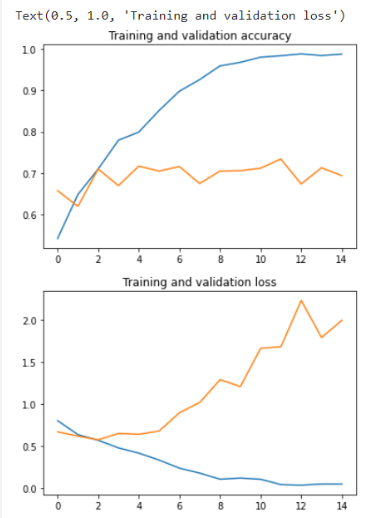
\includegraphics{overfittingCatsDogs.png}
		\\
		The model is \textbf{overfitting} like it's getting out of fashion. The training accuracy (in blue) gets close to 100\% while the validation accuracy (in orange) stalls as 70\%. The validation loss reaches its minimum after only five epochs.\\
		Since you have \textbf{a relatively small number of training examples (2000), overfitting should be the number one concern}. Overfitting happens when a model exposed to too few examples learns patterns that do not generalize to new data, i.e. when the model starts using irrelevant features for making predictions.
		\item \textbf{Week 1 Assignment: Cats vs Dogs}\\
		\begin{minted}{python}
import os
import zipfile
import random
import shutil
import tensorflow as tf
from tensorflow.keras.preprocessing.image import ImageDataGenerator
from shutil import copyfile
import matplotlib.pyplot as plt

# -> Download the dataset
!wget --no-check-certificate \
"https://download.microsoft.com/download/3/E/1/3E1C3F21-ECDB-4869-8368-6DEBA77B919F/kagglecatsanddogs_5340.zip" \
-O "/tmp/cats-and-dogs.zip"
local_zip = '/tmp/cats-and-dogs.zip'
zip_ref   = zipfile.ZipFile(local_zip, 'r')
zip_ref.extractall('/tmp')
zip_ref.close()
source_path = '/tmp/PetImages'
source_path_dogs = os.path.join(source_path, 'Dog')
source_path_cats = os.path.join(source_path, 'Cat')
# Deletes all non-image files (there are two .db files bundled into the dataset)
!find /tmp/PetImages/ -type f ! -name "*.jpg" -exec rm {} +
# os.listdir returns a list containing all files under the given path
print(f"There are {len(os.listdir(source_path_dogs))} images of dogs.")
print(f"There are {len(os.listdir(source_path_cats))} images of cats.")
# Define root directory
root_dir = '/tmp/cats-v-dogs'
# Empty directory to prevent FileExistsError is the function is run several times
if os.path.exists(root_dir):
shutil.rmtree(root_dir)

# -> GRADED FUNCTION: create_train_val_dirs
def create_train_val_dirs(root_path):
	"""
	Creates directories for the train and test sets
	Args:
	root_path (string) - the base directory path to create subdirectories from
	Returns:
	None
	"""
	# Create training and validation directories
	training_dir = os.path.join(root_path, 'training')
	validation_dir = os.path.join(root_path, 'validation')
	# Create subdirectories for cats and dogs under training and validation directories
	os.makedirs(os.path.join(training_dir, 'cats'))
	os.makedirs(os.path.join(training_dir, 'dogs'))
	os.makedirs(os.path.join(validation_dir, 'cats'))
	os.makedirs(os.path.join(validation_dir, 'dogs'))
try:
	create_train_val_dirs(root_path=root_dir)
except FileExistsError:
	print("You should not be seeing this since the upper directory is removed beforehand")
# Test your create_train_val_dirs function
for rootdir, dirs, files in os.walk(root_dir):
	for subdir in dirs:
		print(os.path.join(rootdir, subdir))

# -> GRADED FUNCTION: split_data
def split_data(SOURCE_DIR, TRAINING_DIR, VALIDATION_DIR, SPLIT_SIZE):
	"""
	Splits the data into train and test sets
	Args:
	SOURCE_DIR (string): directory path containing the images
	TRAINING_DIR (string): directory path to be used for training
	VALIDATION_DIR (string): directory path to be used for validation
	SPLIT_SIZE (float): proportion of the dataset to be used for training
	Returns:
	None
	"""
	files = os.listdir(SOURCE_DIR)
	# Filter out files with zero length
	files = [f for f in files if os.path.getsize(os.path.join(SOURCE_DIR, f)) > 0]
	# Shuffle the files
	random.shuffle(files)
	# Determine the split index
	split_idx = int(len(files) * SPLIT_SIZE)
	# Split the files into training and validation sets
	training_files = files[:split_idx]
	validation_files = files[split_idx:]
	# Copy the training files
	for file_name in training_files:
		source = os.path.join(SOURCE_DIR, file_name)
		destination = os.path.join(TRAINING_DIR, file_name)
		copyfile(source, destination)
	# Copy the validation files
	for file_name in validation_files:
		source = os.path.join(SOURCE_DIR, file_name)
		destination = os.path.join(VALIDATION_DIR, file_name)
		copyfile(source, destination)
# Test your split_data function
# Define paths
CAT_SOURCE_DIR = "/tmp/PetImages/Cat/"
DOG_SOURCE_DIR = "/tmp/PetImages/Dog/"
TRAINING_DIR = "/tmp/cats-v-dogs/training/"
VALIDATION_DIR = "/tmp/cats-v-dogs/validation/"
TRAINING_CATS_DIR = os.path.join(TRAINING_DIR, "cats/")
VALIDATION_CATS_DIR = os.path.join(VALIDATION_DIR, "cats/")
TRAINING_DOGS_DIR = os.path.join(TRAINING_DIR, "dogs/")
VALIDATION_DOGS_DIR = os.path.join(VALIDATION_DIR, "dogs/")
# Empty directories in case you run this cell multiple times
if len(os.listdir(TRAINING_CATS_DIR)) > 0:
	for file in os.scandir(TRAINING_CATS_DIR):
		os.remove(file.path)
if len(os.listdir(TRAINING_DOGS_DIR)) > 0:
	for file in os.scandir(TRAINING_DOGS_DIR):
		os.remove(file.path)
if len(os.listdir(VALIDATION_CATS_DIR)) > 0:
	for file in os.scandir(VALIDATION_CATS_DIR):
		os.remove(file.path)
if len(os.listdir(VALIDATION_DOGS_DIR)) > 0:
	for file in os.scandir(VALIDATION_DOGS_DIR):
		os.remove(file.path)
# Define proportion of images used for training
split_size = .9
# Run the function
# NOTE: Messages about zero length images should be printed out
split_data(CAT_SOURCE_DIR, TRAINING_CATS_DIR, VALIDATION_CATS_DIR, split_size)
split_data(DOG_SOURCE_DIR, TRAINING_DOGS_DIR, VALIDATION_DOGS_DIR, split_size)
# Check that the number of images matches the expected output
# Function should perform copies rather than moving images so original directories should contain unchanged images
print(f"\n\nOriginal cat's directory has {len(os.listdir(CAT_SOURCE_DIR))} images")
print(f"Original dog's directory has {len(os.listdir(DOG_SOURCE_DIR))} images\n")
# Training and validation splits
print(f"There are {len(os.listdir(TRAINING_CATS_DIR))} images of cats for training")
print(f"There are {len(os.listdir(TRAINING_DOGS_DIR))} images of dogs for training")
print(f"There are {len(os.listdir(VALIDATION_CATS_DIR))} images of cats for validation")
print(f"There are {len(os.listdir(VALIDATION_DOGS_DIR))} images of dogs for validation")

# -> GRADED FUNCTION: train_val_generators
def train_val_generators(TRAINING_DIR, VALIDATION_DIR):
	"""
	Creates the training and validation data generators
	Args:
	TRAINING_DIR (string): directory path containing the training images
	VALIDATION_DIR (string): directory path containing the testing/validation images
	Returns:
	train_generator, validation_generator - tuple containing the generators
	"""
	# Instantiate the ImageDataGenerator class
	train_datagen = ImageDataGenerator(rescale=1.0/255.)

	# Pass in the appropriate arguments to the flow_from_directory method
	train_generator = train_datagen.flow_from_directory(directory=TRAINING_DIR,
		batch_size=20,
		class_mode='binary',
		target_size=(150, 150))
	# Instantiate the ImageDataGenerator class 
	validation_datagen = ImageDataGenerator(rescale=1.0/255.)
	# Pass in the appropriate arguments to the flow_from_directory method
	validation_generator = validation_datagen.flow_from_directory(directory=VALIDATION_DIR,
		batch_size=20,
		class_mode='binary',
		target_size=(150, 150))
	return train_generator, validation_generator
# Test generators
train_generator, validation_generator = train_val_generators(TRAINING_DIR, VALIDATION_DIR)

# -> GRADED FUNCTION: create_model
def create_model():
	from tensorflow.keras.optimizers import RMSprop
	model = tf.keras.models.Sequential([ 
		tf.keras.layers.Conv2D(16, (3,3), activation='relu', input_shape=(150, 150, 3)),
		tf.keras.layers.MaxPooling2D(2,2),
		tf.keras.layers.Conv2D(32, (3,3), activation='relu'),
		tf.keras.layers.MaxPooling2D(2,2), 
		tf.keras.layers.Conv2D(64, (3,3), activation='relu'), 
		tf.keras.layers.MaxPooling2D(2,2),
		# Flatten the results to feed into a DNN
		tf.keras.layers.Flatten(), 
		# 512 neuron hidden layer
		tf.keras.layers.Dense(512, activation='relu'), 
		# Only 1 output neuron
		tf.keras.layers.Dense(1, activation='sigmoid')  
	])
	model.compile(optimizer=RMSprop(learning_rate=0.001),
		loss='binary_crossentropy',
		metrics=['accuracy']) 
	return model
# Get the untrained model
model = create_model()
# Train the model
# Note that this may take some time.
history = model.fit(train_generator,
	epochs=15,
	verbose=1,
	validation_data=validation_generator)

#-----------------------------------------------------------
# Retrieve a list of list results on training and test data
# sets for each training epoch
#-----------------------------------------------------------
acc=history.history['accuracy']
val_acc=history.history['val_accuracy']
loss=history.history['loss']
val_loss=history.history['val_loss']
epochs=range(len(acc)) # Get number of epochs
#------------------------------------------------
# Plot training and validation accuracy per epoch
#------------------------------------------------
plt.plot(epochs, acc, 'r', "Training Accuracy")
plt.plot(epochs, val_acc, 'b', "Validation Accuracy")
plt.title('Training and validation accuracy')
plt.show()
print("")
#------------------------------------------------
# Plot training and validation loss per epoch
#------------------------------------------------
plt.plot(epochs, loss, 'r', "Training Loss")
plt.plot(epochs, val_loss, 'b', "Validation Loss")
plt.show()
		\end{minted}
		The model is \textbf{overfitting}.
	\end{itemize}
	\subsection{Week 2: Tackle Overfitting with Data Augmentation}
	\begin{itemize}
		\item \textbf{Image augmentation} is a technique used to \textbf{artificially increase the size of a training dataset} by applying various \textbf{transformations} to the original images. This helps in making the model more robust and capable of generalizing well to unseen data.\\
		TensorFlow provides the \textbf{ImageDataGenerator} class, which offers a wide range of image augmentation techniques. It can be used to preprocess images, augment them with various transformations, and feed them into a neural network.\\
		An instance of \textbf{ImageDataGenerator} can be created with desired augmentations as follows:
		\begin{minted}{python}
from tensorflow.keras.preprocessing.image import ImageDataGenerator

train_datagen = ImageDataGenerator(
	rescale=1./255,
	rotation_range=40,
	width_shift_range=0.2,
	height_shift_range=0.2,
	shear_range=0.2,
	zoom_range=0.2,
	horizontal_flip=True,
	fill_mode='nearest'
)
		\end{minted}
		Here's a brief description of some common parameters:
		\begin{itemize}
			\item \textbf{rotation\_range}: Degree range for random rotations.
			\item \textbf{width\_shift\_range}, \textbf{height\_shift\_range}: Range for random horizontal and vertical shifts.
			\item \textbf{shear\_range}: Shear intensity (shear angle in counter-clockwise direction).
			\item \textbf{zoom\_range}: Range for random zoom.
			\item \textbf{horizontal\_flip}: Boolean for randomly flipping half of the images horizontally.
			\item \textbf{fill\_mode}: Points outside the boundaries are filled according to the given mode ('nearest', 'reflect', etc.).
		\end{itemize}
		\item \textbf{Week assignment:}
		The famous \underline{\textbf{cats vs dogs}} dataset to train a model that can classify images of dogs from images of cats. Create a Convolutional Neural Network in Tensorflow and leverage Keras' image preprocessing utilities, more so this time around since Keras provides excellent support for augmenting image data.
		\begin{minted}{python}
	"""
	Should be done!!!
	"""
		\end{minted}
		\speciallink{https://drive.google.com/file/d/1JNBMLpp1g1mV0Si3-v9yWOUR6RE38esN/view?usp=drive_link}{C2W2 notebook} for week's assignment.
	\end{itemize}
	\subsection{Week 3: Transfer Learning}
	\begin{itemize}
		\item \textbf{Transfer Learning:} A powerful technique in deep learning, allowing the use of pre-trained models to accelerate training. TensorFlow simplifies this process.
		\item \textbf{Lab 1:} Transfer Learning\\
		Next code demonstrates the implementation of \textbf{transfer learning} using TensorFlow and the \textbf{InceptionV3} pre-trained model to classify images of cats and dogs.\\ Initially, the pre-trained InceptionV3 model is loaded without the top (fully connected) layer and its weights are set from a downloaded file. The \textbf{convolutional layers of the model are frozen} to retain the pre-trained features, and \textbf{a custom dense network is appended to the base model}. This includes a Flatten layer, a Dense layer with 1024 hidden units and ReLU activation, a \textbf{Dropout layer} with a rate of 0.2 to prevent overfitting, and a final sigmoid activation layer for binary classification.\\
		The model is compiled with the RMSprop optimizer and binary cross-entropy loss function. The dataset of cats and dogs is downloaded and preprocessed with data augmentation techniques for the training set, including rescaling, rotation, width and height shifting, shear transformation, zooming, and horizontal flipping. The validation data is only rescaled.\\
		The model is then trained for 20 epochs with a batch size of 20, using the augmented training data and validation data. Finally, the training and validation accuracy are plotted to visualize the model's performance. The entire code leverages the concept of transfer learning by utilizing a pre-trained model's knowledge and fine-tuning it for a specific task, in this case, classifying cats and dogs, leading to faster training and potentially better performance.
		\begin{minted}{python}
# -> Setup the pretrained model
# Download the pre-trained weights. No top means it excludes the fully connected layer it uses for classification.
!wget --no-check-certificate \
https://storage.googleapis.com/mledu-datasets/inception_v3_weights_tf_dim_ordering_tf_kernels_notop.h5 \
-O /tmp/inception_v3_weights_tf_dim_ordering_tf_kernels_notop.h5

from tensorflow.keras.applications.inception_v3 import InceptionV3
from tensorflow.keras import layers
# Set the weights file you downloaded into a variable
local_weights_file = '/tmp/inception_v3_weights_tf_dim_ordering_tf_kernels_notop.h5'
# Initialize the base model.
# Set the input shape and remove the dense layers.
pre_trained_model = InceptionV3(input_shape = (150, 150, 3), 
	include_top = False, 
	weights = None)
# Load the pre-trained weights you downloaded.
pre_trained_model.load_weights(local_weights_file)
# Freeze the weights of the layers.
for layer in pre_trained_model.layers:
layer.trainable = False

# -> Choose `mixed7` as the last layer of your base model
last_layer = pre_trained_model.get_layer('mixed7')
print('last layer output shape: ', last_layer.output_shape)
last_output = last_layer.output

# -> Add dense layers for your classifier
from tensorflow.keras.optimizers import RMSprop
from tensorflow.keras import Model
# Flatten the output layer to 1 dimension
x = layers.Flatten()(last_output)
# Add a fully connected layer with 1,024 hidden units and ReLU activation
x = layers.Dense(1024, activation='relu')(x)
# Add a dropout rate of 0.2
x = layers.Dropout(0.2)(x)                  
# Add a final sigmoid layer for classification
x = layers.Dense  (1, activation='sigmoid')(x)           
# Append the dense network to the base model
model = Model(pre_trained_model.input, x) 
# Print the model summary. See your dense network connected at the end.
model.summary()

# -> Set the training parameters
model.compile(optimizer = RMSprop(learning_rate=0.0001), 
	loss = 'binary_crossentropy', 
	metrics = ['accuracy'])

# -> Prepare the dataset
# Download the dataset
!wget https://storage.googleapis.com/tensorflow-1-public/course2/cats_and_dogs_filtered.zip
import os
import zipfile
from tensorflow.keras.preprocessing.image import ImageDataGenerator
# Extract the archive
zip_ref = zipfile.ZipFile("./cats_and_dogs_filtered.zip", 'r')
zip_ref.extractall("tmp/")
zip_ref.close()
# Define our example directories and files
base_dir = 'tmp/cats_and_dogs_filtered'
train_dir = os.path.join( base_dir, 'train')
validation_dir = os.path.join( base_dir, 'validation')
# Directory with training cat pictures
train_cats_dir = os.path.join(train_dir, 'cats') 
# Directory with training dog pictures
train_dogs_dir = os.path.join(train_dir, 'dogs') 
# Directory with validation cat pictures
validation_cats_dir = os.path.join(validation_dir, 'cats') 
# Directory with validation dog pictures
validation_dogs_dir = os.path.join(validation_dir, 'dogs')
# Add our data-augmentation parameters to ImageDataGenerator
train_datagen = ImageDataGenerator(rescale = 1./255.,
rotation_range = 40,
width_shift_range = 0.2,
height_shift_range = 0.2,
shear_range = 0.2,
zoom_range = 0.2,
horizontal_flip = True)
# Note that the validation data should not be augmented!
test_datagen = ImageDataGenerator( rescale = 1.0/255. )
# Flow training images in batches of 20 using train_datagen generator
train_generator = train_datagen.flow_from_directory(train_dir,
batch_size = 20,
class_mode = 'binary', 
target_size = (150, 150))     
# Flow validation images in batches of 20 using test_datagen generator
validation_generator =  test_datagen.flow_from_directory( validation_dir,
batch_size  = 20,
class_mode  = 'binary', 
target_size = (150, 150))

# -> Train the model
# Train the model.
history = model.fit(
	train_generator,
	validation_data = validation_generator,
	steps_per_epoch = 100,
	epochs = 20,
	validation_steps = 50,
	verbose = 2)

# -> Evaluate the results
import matplotlib.pyplot as plt
acc = history.history['accuracy']
val_acc = history.history['val_accuracy']
loss = history.history['loss']
val_loss = history.history['val_loss']
epochs = range(len(acc))
plt.plot(epochs, acc, 'r', label='Training accuracy')
plt.plot(epochs, val_acc, 'b', label='Validation accuracy')
plt.title('Training and validation accuracy')
plt.legend(loc=0)
plt.figure()
plt.show()
		\end{minted}
		\item \textbf{Week's assignment:}\\
		Transfer Learning to see if you can increase training accuracy for Horses v Humans. 
		\begin{minted}{python}
	"""
	Should be done!!!
	"""
		\end{minted}
		\speciallink{https://drive.google.com/file/d/16ZbMF6Fvof5xWldWO1TGm0zRj4-4dfV2/view?usp=drive_link}{C2W3 notebook} for week's assignment.		
	\end{itemize}
	\subsection{Week 4: Multiclass Classifications}
	\begin{itemize}
		\item The \textbf{key change} here is the loss function. Whereas before you were using binary\_crossentropy for 2 classes, you will change it to \textbf{categorical\_crossentropy} to extend it to more classes.
		\begin{minted}{python}
model.compile(
	loss = 'categorical_crossentropy',
	optimizer='rmsprop',
	metrics=['accuracy']
)
		\end{minted}
		Prepare the ImageDataGenerator:
		\begin{minted}{python}
from tensorflow.keras.preprocessing.image import ImageDataGenerator

TRAINING_DIR = "tmp/rps-train/rps"
training_datagen = ImageDataGenerator(
	rescale = 1./255,
	rotation_range=40,
	width_shift_range=0.2,
	height_shift_range=0.2,
	shear_range=0.2,
	zoom_range=0.2,
	horizontal_flip=True,
	fill_mode='nearest')

VALIDATION_DIR = "tmp/rps-test/rps-test-set"
validation_datagen = ImageDataGenerator(rescale = 1./255)

train_generator = training_datagen.flow_from_directory(
	TRAINING_DIR,
	target_size=(150,150),
	class_mode='categorical',
	batch_size=126
)

validation_generator = validation_datagen.flow_from_directory(
	VALIDATION_DIR,
	target_size=(150,150),
	class_mode='categorical',
	batch_size=126
)
		\end{minted}
	\item \textbf{Week's assignment:}\\
	Multi-class classification problem using the \textbf{Sign Language MNIST} dataset.
	\begin{minted}{python}
		"""
		Should be done!!!
		"""
	\end{minted}
	\speciallink{https://drive.google.com/file/d/1UUQziZWjyV4i1C4QvsBEBNcJdg-pR\_8s/view?usp=drive\_link}{C2W4 notebook} for week's assignment.		
	\end{itemize}
	\section{C3: Natural Language Processing in TensorFlow}
	\subsection{Week 1: Intro to NLP}
	\begin{itemize}
		\item \textbf{Lab 1: Tokenizer Basics}\\
		\textbf{Generating the vocabulary}
		\begin{minted}{python}
from tensorflow.keras.preprocessing.text import Tokenizer

# Define input sentences
sentences = [
'i love my dog',
'I, love my cat'
]

# Initialize the Tokenizer class
tokenizer = Tokenizer(num_words = 100)

# Generate indices for each word in the corpus
tokenizer.fit_on_texts(sentences)

# Get the indices and print it
word_index = tokenizer.word_index
print(word_index)
		\end{minted}
		\item \textbf{Lab 2: Sequences and Padding}\\
		\textbf{Text to sequences of tokens}
		\begin{minted}{python}
from tensorflow.keras.preprocessing.text import Tokenizer
from tensorflow.keras.preprocessing.sequence import pad_sequences

# Define your input texts
sentences = [
	'I love my dog',
	'I love my cat',
	'You love my dog!',
	'Do you think my dog is amazing?'
]

# Initialize the Tokenizer class
tokenizer = Tokenizer(num_words = 100, oov_token="<OOV>")

# Tokenize the input sentences
tokenizer.fit_on_texts(sentences)

# Get the word index dictionary
word_index = tokenizer.word_index

# Generate list of token sequences
sequences = tokenizer.texts_to_sequences(sentences)

# Print the result
print("\nWord Index = " , word_index)
print("\nSequences = " , sequences)
		\end{minted}
		\textbf{Pad the sequences into a uniform length}
		\begin{minted}{python}
# Pad the sequences to a uniform length
padded = pad_sequences(sequences, maxlen=5, padding='post', truncating='post')

# Print the result
print("\nPadded Sequences:")
print(padded)
		\end{minted}
		\item \textbf{Lab 3: Tokenizing the Sarcasm Dataset}\\
		Load JSON file into my workplace
		\begin{minted}{python}
import json

# Load the JSON file
with open("./sarcasm.json", 'r') as f:
	datastore = json.load(f)
		\end{minted}
		Collect all urls, headlines, and labels for easier processing
		\begin{minted}{python}
# Initialize lists
sentences = [] 
labels = []
urls = []

# Append elements in the dictionaries into each list
for item in datastore:
	sentences.append(item['headline'])
	labels.append(item['is_sarcastic'])
	urls.append(item['article_link'])
		\end{minted}
		Preprocessing the headlines
		\begin{minted}{python}
from tensorflow.keras.preprocessing.text import Tokenizer
from tensorflow.keras.preprocessing.sequence import pad_sequences

# Initialize the Tokenizer class
tokenizer = Tokenizer(oov_token="<OOV>")

# Generate the word index dictionary
tokenizer.fit_on_texts(sentences)

# Print the length of the word index
word_index = tokenizer.word_index
print(f'number of words in word_index: {len(word_index)}')

# Print the word index
print(f'word_index: {word_index}')
print()

# Generate and pad the sequences
sequences = tokenizer.texts_to_sequences(sentences)
padded = pad_sequences(sequences, padding='post')

# Print a sample headline
index = 2
print(f'sample headline: {sentences[index]}')
print(f'padded sequence: {padded[index]}')
print()

# Print dimensions of padded sequences
print(f'shape of padded sequences: {padded.shape}')
		\end{minted}
		\item \textbf{Week's assignment:}\\
		Work with a variation of the \textbf{BBC News Classification Dataset}, which contains 2225 examples of news articles with their respective categories (labels).
		\begin{minted}{python}
			"""
			Should be done!!!
			"""
		\end{minted}
		\speciallink{https://drive.google.com/file/d/1hFbnjZD2dOPpg8sjhsqmuyK4HTFAAGRq/view?usp=drive\_link}{C3W1 notebook} for week's assignment.
	\end{itemize}
	\subsection{Week 2: Word Embeddings}
	\begin{itemize}
		\item \textbf{Lab 1: Training a binary classifier with the IMDB}\\
		\begin{minted}{python}
import tensorflow_datasets as tfds

# -> Load the IMDB Reviews dataset
imdb, info = tfds.load("imdb_reviews", with_info=True, as_supervised=True)

# -> Split the dataset
import numpy as np
# Get the train and test sets
train_data, test_data = imdb['train'], imdb['test']
# Initialize sentences and labels lists
training_sentences = []
training_labels = []
testing_sentences = []
testing_labels = []
# Loop over all training examples and save the sentences and labels
for s,l in train_data:
	training_sentences.append(s.numpy().decode('utf8'))
	training_labels.append(l.numpy())
# Loop over all test examples and save the sentences and labels
for s,l in test_data:
	testing_sentences.append(s.numpy().decode('utf8'))
	testing_labels.append(l.numpy())

# Convert labels lists to numpy array
training_labels_final = np.array(training_labels)
testing_labels_final = np.array(testing_labels)

# -> Generate Padded Sequences
# Parameters
vocab_size = 10000
max_length = 120
embedding_dim = 16
trunc_type='post'
oov_tok = "<OOV>"
from tensorflow.keras.preprocessing.text import Tokenizer
from tensorflow.keras.preprocessing.sequence import pad_sequences
# Initialize the Tokenizer class
tokenizer = Tokenizer(num_words = vocab_size, oov_token=oov_tok)
# Generate the word index dictionary for the training sentences
tokenizer.fit_on_texts(training_sentences)
word_index = tokenizer.word_index
# Generate and pad the training sequences
sequences = tokenizer.texts_to_sequences(training_sentences)
padded = pad_sequences(sequences,maxlen=max_length, truncating=trunc_type)
# Generate and pad the test sequences
testing_sequences = tokenizer.texts_to_sequences(testing_sentences)
testing_padded = pad_sequences(testing_sequences,maxlen=max_length, truncating=trunc_type)

# -> Build and Compile the Model
import tensorflow as tf
# Build the model
model = tf.keras.Sequential([
	tf.keras.layers.Embedding(vocab_size, embedding_dim, input_length=max_length),
	tf.keras.layers.Flatten(),
	tf.keras.layers.Dense(6, activation='relu'),
	tf.keras.layers.Dense(1, activation='sigmoid')
])
# Setup the training parameters
model.compile(loss='binary_crossentropy',optimizer='adam',metrics=['accuracy'])
# Print the model summary
model.summary()

# -> Train the Model
num_epochs = 10
# Train the model
model.fit(padded, training_labels_final, epochs=num_epochs, validation_data=(testing_padded, testing_labels_final))

# -> Visualize Word Embeddings
# Get the embedding layer from the model (i.e. first layer)
embedding_layer = model.layers[0]
# Get the weights of the embedding layer
embedding_weights = embedding_layer.get_weights()[0]
# Print the shape. Expected is (vocab_size, embedding_dim)
print(embedding_weights.shape) 
# Get the index-word dictionary
reverse_word_index = tokenizer.index_word
# loop to generate the files. You will loop vocab_size-1 times, skipping the 0 key because it is just for the padding
import io
# Open writeable files
out_v = io.open('vecs.tsv', 'w', encoding='utf-8')
out_m = io.open('meta.tsv', 'w', encoding='utf-8')
# Initialize the loop. Start counting at `1` because `0` is just for the padding
for word_num in range(1, vocab_size):
	# Get the word associated at the current index
	word_name = reverse_word_index[word_num]
	# Get the embedding weights associated with the current index
	word_embedding = embedding_weights[word_num]
	# Write the word name
	out_m.write(word_name + "\n")
	# Write the word embedding
	out_v.write('\t'.join([str(x) for x in word_embedding]) + "\n")
# Close the files
out_v.close()
out_m.close()
# Now you can go to the Tensorflow Embedding Projector and load the two files
# you downloaded to see the visualization. You can search for words like worst and
# fantastic and see the other words closely located to these.
		\end{minted}
		\item \textbf{Lab 2: Training a binary classifier with the Sarcasm Dataset}
		\begin{minted}{python}
# -> Download dataset
import json
# Load the JSON file
with open("./sarcasm.json", 'r') as f:
datastore = json.load(f)
# Initialize the lists
sentences = []
labels = []
# Collect sentences and labels into the lists
for item in datastore:
	sentences.append(item['headline'])
	labels.append(item['is_sarcastic'])

# -> Hyperparameters
# Number of examples to use for training
training_size = 20000
# Vocabulary size of the tokenizer
vocab_size = 10000
# Maximum length of the padded sequences
max_length = 32
# Output dimensions of the Embedding layer
embedding_dim = 16

# -> Split the dataset
# Split the sentences
training_sentences = sentences[0:training_size]
testing_sentences = sentences[training_size:]
# Split the labels
training_labels = labels[0:training_size]
testing_labels = labels[training_size:]

# -> Preprocessing the train and test sets
import numpy as np
from tensorflow.keras.preprocessing.text import Tokenizer
from tensorflow.keras.preprocessing.sequence import pad_sequences
# Parameters for padding and OOV tokens
trunc_type='post'
padding_type='post'
oov_tok = "<OOV>"
# Initialize the Tokenizer class
tokenizer = Tokenizer(num_words=vocab_size, oov_token=oov_tok)
# Generate the word index dictionary
tokenizer.fit_on_texts(training_sentences)
word_index = tokenizer.word_index
# Generate and pad the training sequences
training_sequences = tokenizer.texts_to_sequences(training_sentences)
training_padded = pad_sequences(training_sequences, maxlen=max_length, padding=padding_type, truncating=trunc_type)
# Generate and pad the testing sequences
testing_sequences = tokenizer.texts_to_sequences(testing_sentences)
testing_padded = pad_sequences(testing_sequences, maxlen=max_length, padding=padding_type, truncating=trunc_type)
# Convert the labels lists into numpy arrays
training_labels = np.array(training_labels)
testing_labels = np.array(testing_labels)

# -> Build and Compile the Model
import tensorflow as tf
# Initialize a GlobalAveragePooling1D (GAP1D) layer
gap1d_layer = tf.keras.layers.GlobalAveragePooling1D()
# Define sample array
sample_array = np.array([[[10,2],[1,3],[1,1]]])
# Print shape and contents of sample array
print(f'shape of sample_array = {sample_array.shape}')
print(f'sample array: {sample_array}')
# Pass the sample array to the GAP1D layer
output = gap1d_layer(sample_array)
# Print shape and contents of the GAP1D output array
print(f'output shape of gap1d_layer: {output.shape}')
print(f'output array of gap1d_layer: {output.numpy()}')

# Build the model
model = tf.keras.Sequential([
tf.keras.layers.Embedding(vocab_size, embedding_dim, input_length=max_length),
tf.keras.layers.GlobalAveragePooling1D(),
tf.keras.layers.Dense(24, activation='relu'),
tf.keras.layers.Dense(1, activation='sigmoid')
])
# Print the model summary
model.summary()

# Compile the model
model.compile(loss='binary_crossentropy',optimizer='adam',metrics=['accuracy'])

# -> Train the Model
num_epochs = 30
# Train the model
history = model.fit(training_padded, training_labels, epochs=num_epochs, validation_data=(testing_padded, testing_labels), verbose=2)

# -> Visualize the Results
import matplotlib.pyplot as plt
# Plot utility
def plot_graphs(history, string):
plt.plot(history.history[string])
plt.plot(history.history['val_'+string])
plt.xlabel("Epochs")
plt.ylabel(string)
plt.legend([string, 'val_'+string])
plt.show()
# Plot the accuracy and loss
plot_graphs(history, "accuracy")
plot_graphs(history, "loss")
		\end{minted}
		\includegraphics{c3w2\_lab2.png}
		\begin{minted}{python}
# -> Visualize Word Embeddings
# using the Tensorflow Embedding Projector
# Get the index-word dictionary
reverse_word_index = tokenizer.index_word
# Get the embedding layer from the model (i.e. first layer)
embedding_layer = model.layers[0]
# Get the weights of the embedding layer
embedding_weights = embedding_layer.get_weights()[0]
# Print the shape. Expected is (vocab_size, embedding_dim)
print(embedding_weights.shape) 

import io
# Open writeable files
out_v = io.open('vecs.tsv', 'w', encoding='utf-8')
out_m = io.open('meta.tsv', 'w', encoding='utf-8')
# Initialize the loop. Start counting at `1` because `0` is just for the padding
for word_num in range(1, vocab_size):
# Get the word associated at the current index
word_name = reverse_word_index[word_num]
# Get the embedding weights associated with the current index
word_embedding = embedding_weights[word_num]
# Write the word name
out_m.write(word_name + "\n")
# Write the word embedding
out_v.write('\t'.join([str(x) for x in word_embedding]) + "\n")
# Close the files
out_v.close()
out_m.close()

# Download the files (???)
files.download('vecs.tsv')
files.download('meta.tsv')
		\end{minted}
		So far, tokenizing datasets from scratch we treating the \textbf{vocab size as a hyperparameter}. Furthermore, we're tokenizing the texts by building a vocabulary of full words. In the next lab, we will make use of a \textbf{pre-tokenized dataset} that uses a vocabulary of subwords.
		\item \textbf{Lab 3: Subword Tokenization with the IMDB Reviews Dataset}\\
		Download the IMDB reviews plain text and tokenized datasets
		\begin{minted}{python}
import tensorflow_datasets as tfds
# Download the plain text default config
imdb_plaintext, info_plaintext = tfds.load("imdb_reviews", with_info=True, as_supervised=True)
# Download the subword encoded pretokenized dataset
imdb_subwords, info_subwords = tfds.load("imdb_reviews/subwords8k", with_info=True, as_supervised=True)
		\end{minted}
		Compare the two datasets
		\begin{minted}{python}
# Print description of features
info_plaintext.features
# Take 2 training examples and print the text feature
for example in imdb_plaintext['train'].take(2):
	print(example[0].numpy())

# Print description of features
info_subwords.features
# Take 2 training examples and print its contents
for example in imdb_subwords['train'].take(2):
	print(example)

# You can get the encoder object included in
# the download and use it to decode the sequences
# Get the encoder
tokenizer_subwords = info_subwords.features['text'].encoder
# Take 2 training examples and decode the text feature
for example in imdb_subwords['train'].take(2):
	print(tokenizer_subwords.decode(example[0]))
		\end{minted}
		Subword Text Encoding
		\begin{minted}{python}
# Get the train set
train_data = imdb_plaintext['train']
# Initialize sentences list
training_sentences = []
# Loop over all training examples and save to the list
for s,_ in train_data:
training_sentences.append(s.numpy().decode('utf8'))

from tensorflow.keras.preprocessing.text import Tokenizer
from tensorflow.keras.preprocessing.sequence import pad_sequences
vocab_size = 10000
oov_tok = '<OOV>'
# Initialize the Tokenizer class
tokenizer_plaintext = Tokenizer(num_words = 10000, oov_token=oov_tok)
# Generate the word index dictionary for the training sentences
tokenizer_plaintext.fit_on_texts(training_sentences)
# Generate the training sequences
sequences = tokenizer_plaintext.texts_to_sequences(training_sentences)
# Decode the first sequence using the Tokenizer class
tokenizer_plaintext.sequences_to_texts(sequences[0:1])
# Total number of words in the word index dictionary
len(tokenizer_plaintext.word_index)
# Print the subwords
print(tokenizer_subwords.subwords)

# Encode the first plaintext sentence using the subword text encoder
tokenized_string = tokenizer_subwords.encode(training_sentences[0])
print(tokenized_string)
# Decode the sequence
original_string = tokenizer_subwords.decode(tokenized_string)
# Print the result
print (original_string)

# Define sample sentence
sample_string = 'TensorFlow, from basics to mastery'
# Encode using the plain text tokenizer
tokenized_string = tokenizer_plaintext.texts_to_sequences([sample_string])
print ('Tokenized string is {}'.format(tokenized_string))
# Decode and print the result
original_string = tokenizer_plaintext.sequences_to_texts(tokenized_string)
print ('The original string: {}'.format(original_string))
# Encode using the subword text encoder
tokenized_string = tokenizer_subwords.encode(sample_string)
print ('Tokenized string is {}'.format(tokenized_string))
# Decode and print the results
original_string = tokenizer_subwords.decode(tokenized_string)
print ('The original string: {}'.format(original_string))

# Show token to subword mapping:
for ts in tokenized_string:
	print ('{} ----> {}'.format(ts, tokenizer_subwords.decode([ts])))
		\end{minted}
		Training the model
		\begin{minted}{python}
BUFFER_SIZE = 10000
BATCH_SIZE = 64
# Get the train and test splits
train_data, test_data = imdb_subwords['train'], imdb_subwords['test'], 
# Shuffle the training data
train_dataset = train_data.shuffle(BUFFER_SIZE)
# Batch and pad the datasets to the maximum length of the sequences
train_dataset = train_dataset.padded_batch(BATCH_SIZE)
test_dataset = test_data.padded_batch(BATCH_SIZE)

import tensorflow as tf
# Define dimensionality of the embedding
embedding_dim = 64
# Build the model
model = tf.keras.Sequential([
	tf.keras.layers.Embedding(tokenizer_subwords.vocab_size, embedding_dim),
	tf.keras.layers.GlobalAveragePooling1D(),
	tf.keras.layers.Dense(6, activation='relu'),
	tf.keras.layers.Dense(1, activation='sigmoid')
])
# Print the model summary
model.summary()

num_epochs = 10
# Set the training parameters
model.compile(loss='binary_crossentropy',optimizer='adam',metrics=['accuracy'])
# Start training
history = model.fit(train_dataset, epochs=num_epochs, validation_data=test_dataset)
		\end{minted}
		Visualize the results
		\begin{minted}{python}
import matplotlib.pyplot as plt

# Plot utility
def plot_graphs(history, string):
	plt.plot(history.history[string])
	plt.plot(history.history['val_'+string])
	plt.xlabel("Epochs")
	plt.ylabel(string)
	plt.legend([string, 'val_'+string])
	plt.show()

# Plot the accuracy and results 
plot_graphs(history, "accuracy")
plot_graphs(history, "loss")
		\end{minted}
		\includegraphics[width=1.2\textwidth]{c3w2\_lab3.png}
		\textbf{Subword text encoding} can be a robust technique to \textbf{avoid out-of-vocabulary tokens}. It can decode uncommon words it hasn't seen before even with a relatively small vocab size. Consequently, it \textbf{results in longer token sequences} when compared to full word tokenization.
		\item \textbf{Week's assignment:}\\
		Not only work with the tokenization process but also create a classifier using specialized layers for text data such as \textbf{Embedding} and \textbf{GlobalAveragePooling1D}.
		\begin{minted}{python}
			"""
			Should be done!!!
			"""
		\end{minted}
		\speciallink{https://drive.google.com/file/d/1MlQPBi9N2OVOV-Sul3QYhBj8vRTqoJ2R/view?usp=drive\_link}{C2W2 notebook} for week's assignment.
	\end{itemize}
	\subsection{Week 3: Sequence models}
	\begin{itemize}
		\item \textbf{Lab 1: Single Layer LSTM (Long Short-Term Memory)}\\
		\textbf{Recurrent Neural Networks} (RNNs) are specialized neural networks designed to process sequential data, with \textbf{connections that loop back on themselves} to maintain memory across the sequence.\\
		\underline{Download the dataset}
		\begin{minted}{python}
import tensorflow_datasets as tfds
# Download the subword encoded pretokenized dataset
dataset, info = tfds.load('imdb_reviews/subwords8k', with_info=True, as_supervised=True)
# Get the tokenizer
tokenizer = info.features['text'].encoder
		\end{minted}
		\underline{Prepare the dataset}
		\begin{minted}{python}
BUFFER_SIZE = 10000
BATCH_SIZE = 256
# Get the train and test splits
train_data, test_data = dataset['train'], dataset['test'], 
# Shuffle the training data
train_dataset = train_data.shuffle(BUFFER_SIZE)
# Batch and pad the datasets to the maximum length of the sequences
train_dataset = train_dataset.padded_batch(BATCH_SIZE)
test_dataset = test_data.padded_batch(BATCH_SIZE)
		\end{minted}
		\underline{Build and compile the model}
		\begin{minted}{python}
import tensorflow as tf
# Hyperparameters
embedding_dim = 64
lstm_dim = 64
dense_dim = 64
# Build the model
model = tf.keras.Sequential([
tf.keras.layers.Embedding(tokenizer.vocab_size, embedding_dim),
tf.keras.layers.Bidirectional(tf.keras.layers.LSTM(lstm_dim)),
tf.keras.layers.Dense(dense_dim, activation='relu'),
tf.keras.layers.Dense(1, activation='sigmoid')
])
# Print the model summary
model.summary()
# Set the training parameters
model.compile(loss='binary_crossentropy', optimizer='adam', metrics=['accuracy'])
		\end{minted}
		\underline{Train the model}\\
		Using the default parameters above, you should reach around 98\% training accuracy and 82\% validation accuracy. 
		\begin{minted}{python}
NUM_EPOCHS = 10
history = model.fit(train_dataset, epochs=NUM_EPOCHS, validation_data=test_dataset)

# PLOT RESULTS
import matplotlib.pyplot as plt
# Plot utility
def plot_graphs(history, string):
plt.plot(history.history[string])
plt.plot(history.history['val_'+string])
plt.xlabel("Epochs")
plt.ylabel(string)
plt.legend([string, 'val_'+string])
plt.show()
# Plot the accuracy and results 
plot_graphs(history, "accuracy")
plot_graphs(history, "loss")
		\end{minted}
	 	\item \textbf{Lab 2: Multiple LSTMs}\\	
	 	\underline{Download and Prepare the Dataset}\\
	 	The same as lab 1.\\
	 	\underline{Build and Compile the Model}\\
	 	You can build \textbf{multiple layer LSTM} models by simply appending another LSTM layer in your Sequential model and enabling the \textit{return\_sequences} flag to \textit{True}. This is because an LSTM layer expects a sequence input so if the previous layer is also an LSTM, then it should output a sequence as well. See the code cell below that demonstrates this flag in action. You'll notice that the output dimension is in 3 dimensions \textit{(batch\_size, timesteps, features)} when when \textit{return\_sequences} is \textit{True}.
	 	\begin{minted}{python}
import tensorflow as tf
import numpy as np
# Hyperparameters
batch_size = 1
timesteps = 20
features = 16
lstm_dim = 8
print(f'batch_size: {batch_size}')
print(f'timesteps (sequence length): {timesteps}')
print(f'features (embedding size): {features}')
print(f'lstm output units: {lstm_dim}')
# Define array input with random values
random_input = np.random.rand(batch_size,timesteps,features)
print(f'shape of input array: {random_input.shape}')
# Define LSTM that returns a single output
lstm = tf.keras.layers.LSTM(lstm_dim)
result = lstm(random_input)
print(f'shape of lstm output(return_sequences=False): {result.shape}')
# Define LSTM that returns a sequence
lstm_rs = tf.keras.layers.LSTM(lstm_dim, return_sequences=True)
result = lstm_rs(random_input)
print(f'shape of lstm output(return_sequences=True): {result.shape}')

import tensorflow as tf
# Hyperparameters
embedding_dim = 64
lstm1_dim = 64
lstm2_dim = 32
dense_dim = 64
# Build the model
model = tf.keras.Sequential([
	tf.keras.layers.Embedding(tokenizer.vocab_size, embedding_dim),
	tf.keras.layers.Bidirectional(tf.keras.layers.LSTM(lstm1_dim,
		return_sequences=True)),
	tf.keras.layers.Bidirectional(tf.keras.layers.LSTM(lstm2_dim)),
	tf.keras.layers.Dense(dense_dim, activation='relu'),
	tf.keras.layers.Dense(1, activation='sigmoid')
])
# Print the model summary
model.summary()

# Set the training parameters
model.compile(loss='binary_crossentropy', optimizer='adam', metrics=['accuracy'])
	 	\end{minted}
 		\item \textbf{Week's assignment:}\\
 		Exploring Overfitting in NLP
 		\begin{minted}{python}
 			"""
 			Should be done!!!
 			"""
 		\end{minted}
 		\speciallink{https://drive.google.com/file/d/1sQOl4BkwqiUkwrYJPIhxUauTC0CikoSN/view?usp=drive\_link}{C3W3 notebook} for week's assignment.		
	\end{itemize}
	\subsection{Week 4: Sequence models and word prediction}
	\begin{itemize}
		\item \textbf{Lab 1: Generating Text with Neural Networks}\\
		\underline{Building the Word Vocabulary}
		\begin{minted}{python}
import tensorflow as tf
import numpy as np 
from tensorflow.keras.layers import Embedding, LSTM, Dense, Bidirectional
from tensorflow.keras.models import Sequential
from tensorflow.keras.preprocessing.text import Tokenizer
from tensorflow.keras.preprocessing.sequence import pad_sequences
from tensorflow.keras.optimizers import Adam

# Load the dataset
data = open('./irish-lyrics-eof.txt').read()
# Lowercase and split the text
corpus = data.lower().split("\n")
# Preview the result
print(corpus)

# Initialize the Tokenizer class
tokenizer = Tokenizer()
# Generate the word index dictionary
tokenizer.fit_on_texts(corpus)
# Define the total words. You add 1 for the index `0` which is just the padding token.
total_words = len(tokenizer.word_index) + 1
print(f'word index dictionary: {tokenizer.word_index}')
print(f'total words: {total_words}')
		\end{minted}
		\underline{Preprocessing the Dataset}\\
		Training sequences and their labels, for example, for the sentence:  "I am using Tensorflow" ->\\
		INPUT              LABEL\\
		-----------------------------\\
		I			---> am\\
		I am		---> using\\
		I am using	---> Tensorflow\\
		Next cell shows how to implement this concept in code. The result would be inputs as padded sequences, and labels as one-hot encoded arrays.
		\begin{minted}{python}
# Initialize the sequences list
input_sequences = []
# Loop over every line
for line in corpus:
	# Tokenize the current line
	token_list = tokenizer.texts_to_sequences([line])[0]
	# Loop over the line several times to generate the subphrases
	for i in range(1, len(token_list)):
		# Generate the subphrase
		n_gram_sequence = token_list[:i+1]
		# Append the subphrase to the sequences list
		input_sequences.append(n_gram_sequence)
# Get the length of the longest line
max_sequence_len = max([len(x) for x in input_sequences])
# Pad all sequences
input_sequences = np.array(pad_sequences(input_sequences, maxlen=max_sequence_len, padding='pre'))
# Create inputs and label by splitting the last token in the subphrases
xs, labels = input_sequences[:,:-1],input_sequences[:,-1]
# Convert the label into one-hot arrays
ys = tf.keras.utils.to_categorical(labels, num_classes=total_words)

# Get sample sentence
sentence = corpus[0].split()
print(f'sample sentence: {sentence}')
# Initialize token list
token_list = []
# Look up the indices of each word and append to the list
for word in sentence: 
	token_list.append(tokenizer.word_index[word])
# Print the token list
print(token_list)

# Pick element
elem_number = 6
# Print token list and phrase
print(f'token list: {xs[elem_number]}')
print(f'decoded to text: {tokenizer.sequences_to_texts([xs[elem_number]])}')
# Print label
print(f'one-hot label: {ys[elem_number]}')
print(f'index of label: {np.argmax(ys[elem_number])}')
		\end{minted}
		\underline{Build the Model}\\
		\begin{minted}{python}
# Hyperparameters
embedding_dim = 100
lstm_units = 150
learning_rate = 0.01
# Build the model
model = Sequential([
	Embedding(total_words, embedding_dim, input_length=max_sequence_len-1),
	Bidirectional(LSTM(lstm_units)),
	Dense(total_words, activation='softmax')
])
# Use categorical crossentropy because this is a multi-class problem
model.compile(
	loss='categorical_crossentropy', 
	optimizer=tf.keras.optimizers.Adam(learning_rate=learning_rate), 
	metrics=['accuracy']
)
# Print the model summary
model.summary()
		\end{minted}
		\underline{Train the model}
		\begin{minted}{python}
# Train the model
history = model.fit(xs, ys, epochs=500)
		\end{minted}
		\underline{Visualize the results}
		\begin{minted}{python}
import matplotlib.pyplot as plt
# Plot utility
def plot_graphs(history, string):
	plt.plot(history.history[string])
	plt.xlabel("Epochs")
	plt.ylabel(string)
	plt.show()
# Visualize the accuracy
plot_graphs(history, 'accuracy')
		\end{minted}
		\underline{Generating Text}\\
		1. Feed a seed text to initiate the process.\\
		2. Model predicts the index of the most probable next word.\\
		3. Look up the index in the reverse word index dictionary.\\
		4. Append the next word to the seed text.\\
		5. Feed the result to the model again.
		\begin{minted}{python}
# Define seed text
seed_text = "Laurence went to Dublin"
# Define total words to predict
next_words = 100
# Loop until desired length is reached
for _ in range(next_words):
	# Convert the seed text to a token sequence
	token_list = tokenizer.texts_to_sequences([seed_text])[0]
	# Pad the sequence
	token_list = pad_sequences([token_list], maxlen=max_sequence_len-1, padding='pre')
	# Feed to the model and get the probabilities for each index
	probabilities = model.predict(token_list)
	# Get the index with the highest probability
	predicted = np.argmax(probabilities, axis=-1)[0]
	# Ignore if index is 0 because that is just the padding.
	if predicted != 0:
		# Look up the word associated with the index. 
		output_word = tokenizer.index_word[predicted]
		# Combine with the seed text
		seed_text += " " + output_word
# Print the result	
print(seed_text)
		\end{minted}
		Frequent repetition of words the longer the sentence gets. There are ways to get around it and the next cell shows one. Basically, instead of getting the index with max probability, you will get the top three indices and choose one at random. See if the output text makes more sense with this approach.
		\begin{minted}{python}
# Define seed text
seed_text = "Laurence went to Dublin"
# Define total words to predict
next_words = 100
# Loop until desired length is reached
for _ in range(next_words):
	# Convert the seed text to a token sequence
	token_list = tokenizer.texts_to_sequences([seed_text])[0]
	# Pad the sequence
	token_list = pad_sequences([token_list], maxlen=max_sequence_len-1, padding='pre')
	# Feed to the model and get the probabilities for each index
	probabilities = model.predict(token_list)
	# Pick a random number from [1,2,3]
	choice = np.random.choice([1,2,3])
	# Sort the probabilities in ascending order 
	# and get the random choice from the end of the array
	predicted = np.argsort(probabilities)[0][-choice]
	# Ignore if index is 0 because that is just the padding.
	if predicted != 0:
		# Look up the word associated with the index. 
		output_word = tokenizer.index_word[predicted]
		# Combine with the seed text
		seed_text += " " + output_word
# Print the result	
print(seed_text)
		\end{minted}
		This lab is a first look at preparing data and building a model for text generation.\\
		\item \textbf{Week's assignment:}\\
		Create a model that will predict the next word in a text sequence using a corpus of Shakespeare's sonnets.
		\begin{minted}{python}
			"""
			Should be done!!!
			"""
		\end{minted}
		\speciallink{https://drive.google.com/file/d/173BJXUhqEiVZcDve6qjLl98AQPyrJvWQ/view?usp=drive\_link}{C3W4 notebook} for week's assignment.
	\end{itemize}	
	\section{C4: Sequences, Time Series and Prediction in TensorFlow}
	\subsection{Week 1: Sequences and Prediction}
	\begin{itemize}
		\item \speciallink{https://community.deeplearning.ai/t/tf1-course-4-lecture-notes/121711}{TF1 Course 4: Lecture Notes}
		\item \textbf{Time Series Forecasting}\\
		\textbf{Naive Forecasting}: A simple method where the next value is assumed to be the same as the last value. It can serve as a baseline and sometimes performs surprisingly well.\\
		\textbf{Measuring Performance}: To evaluate the forecasting model, the time series is typically split into training, validation, and test periods. This is known as fixed partitioning.\\
		\textbf{Seasonality Consideration}: If the time series has seasonality, each period should contain a whole number of seasons (e.g., one year, two years) to avoid uneven representation of months.\\
		\textbf{Training and Validation Process}: Train the model on the training period and evaluate it on the validation period to find the right architecture and hyperparameters.\\
		\textbf{Retraining with Test Data}: Once satisfied with the performance, the model can be retrained using both training and validation data, and then tested on the test period. Sometimes, retraining with test data is done as it's the closest data to the current point in time.\\
		\textbf{Roll-Forward Partitioning}: An alternative to fixed partitioning, where the training period is gradually increased (e.g., by one day or one week at a time), and the model is continually refined.\\
		\item \textbf{Moving Average Forecasting}: A method that calculates the average of values over a fixed period (e.g., 30 days). It eliminates noise but does not anticipate trend or seasonality.\\
		\textbf{Differencing Technique}: To avoid the limitations of moving average, the trend and seasonality can be removed by studying the difference between the value at time T and an earlier period (e.g., a year earlier).\\
		\textbf{Final Forecasts}: The forecasts for the original time series are obtained by adding back the value at time T minus 365, resulting in improved forecasts.\\
		\textbf{Noise Reduction}: The final forecasts may still contain noise from past values. This can be further smoothed by applying a moving average to the past values, leading to even better results.\\
		\textbf{Simple vs. Complex Models}: Simple approaches like \textbf{moving averages} can sometimes be highly effective, and deep learning or more complex models may not always be necessary.
		\item \textbf{Week's assignment:}\\
		Work with time series data. All of the data is generated and the task is to implement several functions to split the data, create forecasts and evaluate the quality of those forecasts.
		\begin{minted}{python}
			"""
			Should be done!!!
			"""
		\end{minted}
		\speciallink{https://drive.google.com/file/d/1wYCVYszbeBfWRB6kX9NINBWFseD8nd59/view?usp=drive\_link}{C4W1 notebook} for week's assignment.		
	\end{itemize}
	\subsection{Week 2: Statistical and Deep Learning Approaches to Time Series Forecasting}
	\begin{itemize}
		\item \textbf{Lab 1: Preparing Time Series Features and Labels}
		\begin{minted}{python}
	"""
	Lab 1 Code here
	"""
		\end{minted}
		\item \textbf{Lab 2: Training a Single Layer Neural Network with Time Series Data}
		\begin{minted}{python}
	"""
	Lab 2 Code here
	"""
		\end{minted}
		\item \textbf{Lab 3: Training a Deep Neural Network with Time Series Data}
		\begin{minted}{python}
	"""
	Lab 3 Code here
	"""
		\end{minted}
		\item \textbf{Week's assignment:}\\
		Predicting time series
		\begin{minted}{python}
			"""
			Should be done!!!
			"""
		\end{minted}
		\speciallink{https://drive.google.com/file/d/18-VdKy39XDuRYdZipjfkXdUX1iXD2Kd8/view?usp=drive\_link}{C4W2 notebook} for week's assignment.
	\end{itemize}
	\subsection{Week 3: Recurrent Neural Networks for Time Series}
	\begin{itemize}
		\item \textbf{Lab 1: Using a Simple RNN for forecasting}
		\begin{minted}{python}
			"""
			Lab 1 of C4W3 code here
			"""
		\end{minted}
		\item \textbf{Lab 2: Using a multi-layer LSTM for forecasting}
		\begin{minted}{python}
			"""
			Lab 2 of C4W3 code here
			"""
		\end{minted}
		\item \textbf{Week's assignment:}\\
		Forecast using RNNs or LSTMs
		\begin{minted}{python}
			"""
			Should be done!!!
			"""
		\end{minted}
		\speciallink{https://drive.google.com/file/d/1PVYDPLobYhiSQvCLlvr\_\_akvsRclDYGH/view?usp=drive\_link}{C4W3 notebook} for week's assignment.
	\end{itemize}
	\subsection{Week 4: Real-world time series data}
	\begin{itemize}
		\item \textbf{Lab 1: Using Convolutions with LSTMs}
		\begin{minted}{python}
			"""
			Lab 1 of C4W4 code here
			"""
		\end{minted}
		\item \textbf{Lab 2: Predicting Sunspots with Neural Networks (DNN only)}
		\begin{minted}{python}
			"""
			Lab 2 of C4W4 code here
			"""
		\end{minted}
		\item \textbf{Lab 3: Predicting Sunspots with Neural Networks (combined layers)}
		\begin{minted}{python}
			"""
			Lab 3 of C4W4 code here
			"""
		\end{minted}
		\item \textbf{Week's assignment:}\\
		Using real world data, using Tensorflow's layers for processing sequence data such as Recurrent layers or LSTMs you will also use Convolutional layers to improve the model's performance.
		\begin{minted}{python}
			"""
			Should be done!!!
			"""
		\end{minted}
		\speciallink{https://drive.google.com/file/d/12EXkB7wgNFRVr0u6Xxty354503HDtgUc/view?usp=drive\_link}{C4W4 notebook} for week's assignment.
	\end{itemize}


%\item \textbf{Week's assignment:}\\
%*short description___
%\begin{minted}{python}
%	"""
%	Should be done!!!
%	"""
%\end{minted}
%\speciallink{*link___}{C_W_ notebook} for week's assignment.
\end{document}